%% Equations of straight lines %%
% Question 5
\question Find the equation of the lines described below. 
Give the equation in the form:
\[
	ax + by + c = 0
\]
where $a$, $b$ and $c$ are whole numbers and $a > 0$.
\begin{parts}
	\part line in Exercise 2 (b)
		\begin{solution}
			\[
				y = -2x + 1
			\]
			\qSolMath{
				2x + y - 1 = 0
			}{}
		\end{solution}

	\part line in Exercise 2 (e)
		\begin{solution}
			\[
				y = -\frac{3}{4}x + \frac{1}{2}
			\]
			\qSolMath{
				3x + 4y - 2 = 0
			}{}
		\end{solution}
		
	\part line in Exercise 3 (c)
		\begin{solution}
			\[
				y = \frac{2}{5}x -3
			\]
			\qSolMath{
				2x - 5y - 15 = 0
			}{}
		\end{solution}
	
	\part line in Exercise 4 (b)
		\begin{solution}
			\[
				y = -3x + 4
			\]
			\qSolMath{
				3x + y - 4 = 0
			}{}
		\end{solution}	
	% e-h
	\part line in Exercise 4 (d)
		\begin{solution}
			\[
				y = -\frac{1}{2}x + 2
			\]
			\qSolMath{
				x + 2y - 4 = 0
			}{}
		\end{solution}	
	
	\part line in Exercise 4 (e)
		\begin{solution}
			\[
				y = -2x - 1
			\]
			\qSolMath{
				2x + y + 1 = 0
			}{}
		\end{solution}	

	\part line through $(3, -2)$ and $(3,2)$
		\begin{solution}
			\par
			Trying the same approach as previous questions\dots
			\[
				\frac{y-y_{1}}{y_{2}-y_{1}} = \frac{x-x_{1}}{x_{2}-x{1}}
			\]
			\[
				\rightarrow
				\frac{y-(-2)}{2-(-2)} = \frac{x-3}{3-3}
			\]
			\[
				\frac{y+2}{4} = \frac{x-3}{0}
			\]
			\[
				\rightarrow
				\text{undefined.}
			\]
			Oh no. If the approach we have previously been using doesn't work
			let's try another tack.
			\newline
			Let's plot the two points\dots
			\begin{center}
			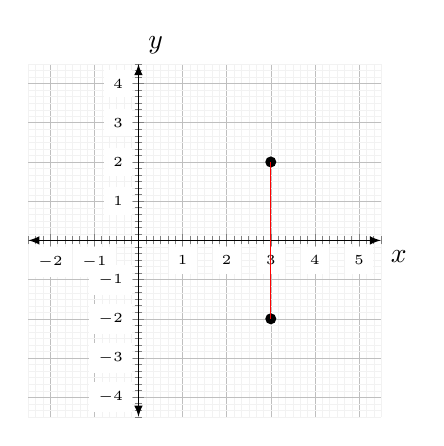
\begin{tikzpicture}
				\begin{axis}[
						width=0.5\textwidth,
						height=0.5\textwidth,
						xtick distance=1,
						ytick distance=1,
						xmin=-2,xmax=5,
						ymin=-4,ymax=4,
						xlabel = $x$,
						ylabel = $y$,
						grid=both,
						grid style={line width=.1pt, draw=gray!10},
						major grid style={line width=.2pt,draw=gray!50},
						axis lines=middle,
						minor tick num=5,
						enlargelimits={abs=0.5},
						axis line style={latex-latex},
						ticklabel style={font=\tiny,fill=white},
						xlabel style={at={(ticklabel* cs:1)},anchor=north west},
						ylabel style={at={(ticklabel* cs:1)},anchor=south west},
						legend pos=north east,
						% legend entries={
						% 	$y = -\frac{1}{3}x + \frac{10}{3}$,
						% 	$y = 3x$,
						% },
						legend cell align={left},
					]
					% points
					\fill (axis cs: 3, -2) circle[radius=2pt];
					\fill (axis cs: 3, 2) circle[radius=2pt];
					\addplot[color=red] table[row sep = crcr]{3 -2 \\ 3 2 \\};
				\end{axis}
			\end{tikzpicture}
			\end{center}
			The x-coordinate does not change and we have a straight vertical 
			line. From theory this line will be of the type,
			\[
				ax + c = 0
			\]
			From visual inspection $x=3$ at all points $\therefore$
			\par
			\qSolMath{
				x - 3 = 0
			}{}
		\end{solution}
	
	\part the vertical line passing through the point 
	$\left( 0, \frac{2}{3} \right)$
		\begin{solution}
			For vertical lines the x-coordinate does not change, we can pick
			any y-coordinate for the second point. Let's pick $(0,0)$ to make
			life easy
			\[
				\frac{y-y_{1}}{y_{2}-y_{1}} = \frac{x-x_{1}}{x_{2}-x{1}}
			\]
			\[
				\rightarrow
				\frac{y-(3)}{0-(3)} = \frac{x-0}{0-0}
			\]
			\[
				\rightarrow
				\text{undefined.}
			\]
			Plotting the two points\dots
			\begin{center}
			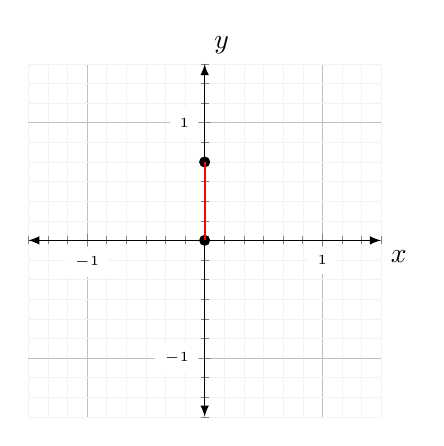
\begin{tikzpicture}
				\begin{axis}[
						width=0.5\textwidth,
						height=0.5\textwidth,
						xtick distance=1,
						ytick distance=1,
						xmin=-1,xmax=1,
						ymin=-1,ymax=1,
						xlabel = $x$,
						ylabel = $y$,
						grid=both,
						grid style={line width=.1pt, draw=gray!10},
						major grid style={line width=.2pt,draw=gray!50},
						axis lines=middle,
						minor tick num=5,
						enlargelimits={abs=0.5},
						axis line style={latex-latex},
						ticklabel style={font=\tiny,fill=white},
						xlabel style={at={(ticklabel* cs:1)},anchor=north west},
						ylabel style={at={(ticklabel* cs:1)},anchor=south west},
						legend pos=north east,
						% legend entries={
						% 	$y = -\frac{1}{3}x + \frac{10}{3}$,
						% 	$y = 3x$,
						% },
						legend cell align={left},
					]
					% points
					\fill (axis cs: 0, 2/3) circle[radius=2pt];
					\fill (axis cs: 0, 0) circle[radius=2pt];
					\addplot[
						color=red,
						thick,
						] table[row sep = crcr]{0 0 \\ 0 0.666 \\};
				\end{axis}
			\end{tikzpicture}
			\end{center}
			From theory this line will be of the type,
			\[
				ax + c = 0
			\]
			From visual inspection $x=0$ at all points $\therefore$
			\par
			\qSolMath{
				x = 0
			}{}
		\end{solution}

\end{parts}

\appenddata{questionSolutions}{
{
\begin{parts}
	\part $2x + y - 1 = 0$
	\part $3x + 4y - 2 = 0$
	\part $2x - 5y - 15 = 0$
	\part $3x + y - 4 = 0$
	% e-h
	\part $x + 2y - 4 = 0$
	\part $2x + y + 1 = 0$
	\part $x - 3 = 0$
	\part $x = 0$
\end{parts}
}
}